\documentclass[11pt, twocolumn]{article}

\usepackage[spanish]{babel}
\usepackage[none]{hyphenat}
\usepackage[left=1.5cm, right=1.5cm, top = 2cm, bottom=2.5cm]{geometry}
\usepackage{parskip}
\usepackage[export]{adjustbox}
\usepackage{enumitem}
\usepackage{listings}
\usepackage{color}
\usepackage{fancyhdr}
\usepackage{graphicx}
\usepackage{caption}
% \usepackage{subcaption}
% \usepackage{wrapfig}
% \usepackage{longtable}
% \usepackage{multirow, makecell}
% \usepackage{amsmath} 
\usepackage[hidelinks]{hyperref}
\usepackage{csquotes}

\newcommand{\linejump}{\hfill \break}
\renewcommand{\thefootnote}{\fnsymbol{footnote}}
% \newcommand{\unit}[1]{\ensuremath{\, \mathrm{#1}}}

\definecolor{dkgreen}{rgb}{0,0.6,0}
\definecolor{gray}{rgb}{0.5,0.5,0.5}
\definecolor{mauve}{rgb}{0.58,0,0.82}
\lstset{
  language=Java,
  aboveskip=3mm,
  belowskip=3mm,
  showstringspaces=false,
  columns=flexible,
  basicstyle={\tiny\ttfamily},
  numbers=none,
  numberstyle=\tiny\color{gray},
  keywordstyle=\color{blue},
  commentstyle=\color{dkgreen},
  stringstyle=\color{mauve},
  breaklines=true,
  breakatwhitespace=true,
  tabsize=2
}

\sloppy
\setlength{\parindent}{0cm}
\setlength{\columnsep}{0.5cm}
\decimalpoint
\graphicspath{{img/}}

\hypersetup{colorlinks=true, urlcolor=blue, citecolor=blue}
\urlstyle{same}

\pagestyle{fancyplain}
\fancyhf{}
\fancyhead[L]{\scriptsize 
  Universidad Nacional Autónoma de México \\
  Laboratorio de Programación Orientada a Objetos \\
  M.C. Leonardo Ledesma Dominguez
}
\fancyhead[R]{\thepage}


\begin{document}
  \twocolumn[
    \centering
    Acosta Porcayo Alan Omar, Gutiérrez Grimaldo Alejandro, Medina Villa Samuel

    \linejump

    \LARGE \textbf{Práctica 5. Abstracción y Encapsulamiento} \\
    
    \linejump
  ]
      
  \footnotetext{
    \scriptsize 
    Acosta Porcayo Alan Omar Ing. en Computación 320206102 \\
    Gutiérrez Grimaldo Alejandro Ing. en Computación 320282098 \\
    Medina Villa Samuel Ing. en Computación 320249538
  }
        
  \fancyfoot{}

  \section*{Resumen}
  Esta práctica se enfoca en comprender las características y funciones principales de un objeto y examinar cómo utilizar diferentes niveles de acceso a estas características. Se investigará a fondo el objeto y se evaluará su versatilidad en función de los diferentes niveles de acceso. Los resultados proporcionarán información valiosa sobre la importancia de comprender un objeto a fondo y cómo esto puede afectar su utilidad y diseño.

  \section*{Introducción}
  La abstracción y el encapsulamiento son dos conceptos fundamentales en la programación orientada a objetos que permiten simplificar y proteger la complejidad de los sistemas. La abstracción se enfoca en centrarse en lo que un objeto hace sin preocuparse por cómo lo hace, lo que facilita la comprensión y el uso de objetos complejos. Por otro lado, el encapsulamiento implica ocultar los detalles internos de un objeto y proporcionar acceso controlado a sus datos y operaciones a través de métodos.

  \subsection*{Abstracción}
  La abstracción se refiere a la capacidad de enfocarse en los aspectos más significativos de un problema y expresar una solución en términos simplificados. Esto permite manejar la complejidad de los sistemas del mundo real al analizar ``qué hace'' un objeto en lugar de ``cómo lo hace''. La abstracción se ilustra con un ejemplo común: la televisión, cuyos usuarios pueden interactuar con sus funciones sin necesidad de conocer su funcionamiento interno.

  \subsection*{Encapsulamiento}
  El encapsulamiento implica agrupar datos y operaciones relacionadas dentro de una unidad de programación, protegiendo así la información interna de un objeto. Esto se logra mediante el ocultamiento de datos, lo que significa que el acceso a los atributos de un objeto se realiza a través de métodos específicos. Los niveles de visibilidad, como público, protegido y privado, controlan qué partes del programa pueden acceder a estos atributos, proporcionando una interfaz clara para interactuar con el objeto.

  \subsection*{Modificadores de Acceso}
  Los modificadores de acceso, como público, protegido y privado, definen la visibilidad de los miembros de una clase (atributos y métodos). Estos modificadores permiten controlar quién puede acceder y modificar los atributos de un objeto. El uso adecuado de estos modificadores garantiza la integridad de los datos y facilita futuros cambios en la implementación sin afectar a otras partes del programa.

  \subsection*{Acceso a Miembros}
  Los métodos de acceso, como \textit{getters} y \textit{setters}, son métodos públicos que permiten leer y modificar los atributos privados de un objeto. Los métodos consultores (\textit{getters}) proporcionan información sin cambiar los valores de los atributos, mientras que los métodos modificadores (\textit{setters}) permiten cambiar esos valores. Esta separación de acceso controlado a los datos internos mejora la modularidad y la seguridad del código.

  \subsection*{Composición}
  La composición es la capacidad de una clase de tener referencias a objetos de otras clases como miembros. Esto refleja las relaciones ``tiene un'' en sistemas complejos. Por ejemplo, un cuerpo humano tiene un cerebro y un corazón. La composición facilita la reutilización de software y la construcción de sistemas jerárquicos y modularizados.

  En conjunto, la abstracción y el encapsulamiento son principios clave para crear sistemas de software eficientes y mantenibles, permitiendo una comprensión más clara de objetos complejos y protegiendo la integridad de los datos y la funcionalidad del programa.

  \section*{Objetivos}
  \begin{itemize}
    \item Aplicar el concepto de abstracción para el diseño de clases que integran una solución, utilizando el encapsulamiento para proteger la información y ocultar la implementación.
    \item Crear clases que representen abstracciones significativas de componentes o entidades del sistema, centrándose en sus características clave y funcionalidades sin preocuparse por los detalles de implementación.
    \item Implementar el encapsulamiento en las clases, asegurando que los datos internos estén protegidos de modificaciones no autorizadas, y permitiendo el acceso controlado a través 
  \end{itemize}

  \section*{Metodología} 
  \subsection*{Ejercicio realizado por el profesor}
  Ejemplo de uso de interfaces. 

  \textbf{Código}
  \begin{lstlisting}
interface Poligono {
  // firma de metodos
  void getArea(int a, int b);
}  

class Rectangulo implements Poligono {
  // implementacion del metodo de la interfaz
  public void getArea(int a, int b) {
    System.out.println("El area del rectangulo es: " + (a * b));
  }
}

class Main {
  public static void main(String[] args) {
    Rectangulo r = new Rectangulo();
    r.getArea(4, 8);
  }
}  
  \end{lstlisting}

  Recreación del juego ``Gato''.
  \begin{lstlisting}
import java.util.*;

interface Board {
  // En interfaz por lo general los metodos son default
  String checkWinner();
  void printBoard();
}

public class TicTacToe implements Board {
  static String[] board;
  static String player; // Posible objeto que venga de la clase Player L11
    
  // Override
  public String checkWinner() {
    for(int i = 0;  i <8; i ++) {
      String line = null;
      switch(i) {
        case 0: line = board[0] + board[1] + board[2]; break;
        case 1: line = board[3] + board[4] + board[5]; break;
        case 2: line = board[6] + board[7] + board[8]; break;
        case 3: line = board[0] + board[3] + board[6]; break;
        case 4: line = board[1] + board[4] + board[7]; break;
        case 5: line = board[2] + board[5] + board[8]; break;
        case 6: line = board[0] + board[4] + board[8]; break;
        case 7: line = board[2] + board[4] + board[6]; break;
      }

      if(line.equals("XXX")) // Si gana el jugador X
				return "X";
			else if(line.equals("OOO")) // Si gana el jugador O
				return "O";
    }

    for(int a = 0; a < 9; a ++) {
      if(Arrays.asList(board).contains(String.valueOf(a + 1)))
          break;
      else if(a==8)
          return "DRAW";
    }

    System.out.println("\nEs el turneo de " + player + ", ingrese una casilla: ");

    return null;
  }

  //imprimir
  /*
  |-------|-------|-------|
  |	  1	  |	  2  	|  	3  	|
  |-------|-------|-------|
  |	  4	  |	  5	  |	  6	  |
  |-------|-------|-------|
  |	  7	  |	  8  	|  	9  	|
  */

  public void printBoard() {
    System.out.println("\n|---|---|---|");
    System.out.println("| " + board[0] + " | " + board[1] + " | " + board[2] + " |");
    System.out.println("|---|---|---|");
    System.out.println("| " + board[3] + " | " + board[4] + " | " + board[5] + " |");
    System.out.println("|---|---|---|");
    System.out.println("| " + board[6] + " | " + board[7] + " | " + board[8] + " |");
    System.out.println("|---|---|---|");
  }

  public static void main(String[] args) {
    Scanner in = new Scanner(System.in);
    board = new String[9];
    player = "X";
    String winner = null;

    TicTacToe t = new TicTacToe();

    // Llenar la matriz board
    for(int i=0;i<9;i++)
      board[i] = String.valueOf(i+1);

    System.out.println("Bienvenido Tic Tac Toe 3x3");

    t.printBoard();

    System.out.println("Es el turneo de " + player + ", ingrese una casilla: ");
    while(winner == null) {
      int numSlot;

      numSlot = in.nextInt();
      if(!(numSlot>0 && numSlot<=9)) {
        System.out.println("Opcion no valida");
        continue;
      }

      if(board[numSlot-1].equals(String.valueOf(numSlot))) {
        board[numSlot-1] = player; // Player vale "X"
        if(player.equals("X"))
          player = "O";
        else
          player = "X";
        t.printBoard();
        winner = t.checkWinner();
      } else
        System.out.println("El slot ya esta ocupado");
    }

    if(winner.equals("DRAW"))
      System.out.println("Nadie gana. Gracias por jugar");
    else 
      System.out.println("Ganaste " + winner + " eres un PRO");

    in.close();
  }
}
  \end{lstlisting}

  \section*{Resultados}
  \subsection*{Problema 1}
  Modifique el programa de \textit{Tic Tac Toe} haciendo: 
  \begin{enumerate}[label=\alph*.]
    \item El Juego de $5\times 5$ y el que gane lo haga con $4$ símbolos unidos.
    \item Cree una clase abstracta que sea el jugador (X-O) y herede la clase principal.
  \end{enumerate}
  \textbf{\textit{Implementar la herencia hibrida, usar interfaces y clases abstractas.}}

  \linejump
  \textbf{Explicación} \\
  Este código representa una adaptación del juego ``Tic Tac Toe'' en una versión ampliada de 5x5, en la que dos jugadores se enfrentan para conseguir una fila, columna o diagonal con cuatro símbolos, ``X'' u ``O'', antes que su oponente.

  En esta versión, el tablero se representa mediante una matriz de 5x5 llamada \textit{board}. Inicialmente, todas las casillas están numeradas del 1 al 25, indicando las posiciones iniciales del juego.

  Los jugadores se identifican mediante objetos de la clase \textit{HumanPlayer}, uno para ``X'' (denominado \textit{playerX}) y otro para ``O'' (denominado \textit{playerO}). Estos jugadores se alternan en cada turno para realizar sus respectivos movimientos en el tablero.

  La ejecución del juego ocurre en el método \textit{main()}. Un bucle \textit{while} se mantiene en funcionamiento hasta que se declare un ganador o se produzca un empate. En cada turno, se muestra el estado actual del tablero, y el jugador en turno elige una casilla válida para colocar su símbolo. El juego verifica si el movimiento es válido y si la casilla está disponible antes de actualizar el tablero y pasar al siguiente turno.

  La lógica para determinar un ganador se encuentra en el método \textit{checkWinner()}, que examina todas las posibles combinaciones de filas, columnas y diagonales para verificar si algún jugador ha obtenido la victoria. En caso contrario, si no quedan casillas vacías, se declara un empate.
  
  Finalmente, una vez que el juego ha llegado a su conclusión, se muestra el resultado en la consola, indicando si hubo un ganador o si el juego culminó en empate.

  \textbf{Clase \textit{HumanPlayer}}
  \begin{lstlisting}
import java.util.*;

abstract class Player {
  protected String symbol;

  public abstract void setSymbol(String symbol);
  public abstract int makeMove();
}

class HumanPlayer extends Player {
  Scanner scanner = new Scanner(System.in);

  public HumanPlayer(String symbol) {
    setSymbol(symbol);
  }

  @Override
  public void setSymbol(String symbol) {
    this.symbol = symbol;
  }

  @Override
  public int makeMove() {
    System.out.print("Es el turno de " + this.symbol);
    System.out.print(". Ingresa un numero del 1 al 25: ");
    int move = scanner.nextInt();
    return move;
  }
}
  \end{lstlisting}

  \textbf{Clase \textit{TicTacToe}}
  \begin{lstlisting}
interface Board {
  String checkWinner();
  void printBoard();
}

public class TicTacToe implements Board {
  private static String[] board = new String[25];
  private static HumanPlayer playerX = new HumanPlayer("X");
  private static HumanPlayer playerO = new HumanPlayer("O");

  public TicTacToe() {
    for (int i = 0; i < 9; i ++) {
        board[i] = "0" + String.valueOf(i + 1);
    }
    for (int i = 9; i < 25; i++) {
        board[i] = String.valueOf(i + 1);
    }
  }

  public String checkWinner() {
    for (int i = 0; i < 5; i++) {
      for (int j = 0; j < 5; j++) {
        if (j + 3 < 5) {
          if (board[i * 5 + j].equals(board[i * 5 + j + 1]) &&
              board[i * 5 + j].equals(board[i * 5 + j + 2]) &&
              board[i * 5 + j].equals(board[i * 5 + j + 3])) {
            return board[i * 5 + j];
          }
        }
        if (i + 3 < 5) {
          if (board[i * 5 + j].equals(board[(i + 1) * 5 + j]) &&
              board[i * 5 + j].equals(board[(i + 2) * 5 + j]) &&
              board[i * 5 + j].equals(board[(i + 3) * 5 + j])) {
            return board[i * 5 + j];
          }
        }
        if (i + 3 < 5 && j + 3 < 5) {
          if (board[i * 5 + j].equals(board[(i + 1) * 5 + j + 1]) &&
              board[i * 5 + j].equals(board[(i + 2) * 5 + j + 2]) &&
              board[i * 5 + j].equals(board[(i + 3) * 5 + j + 3])) {
            return board[i * 5 + j];
          }
        }
        if (i + 3 < 5 && j - 3 >= 0) {
          if (board[i * 5 + j].equals(board[(i + 1) * 5 + j - 1]) &&
              board[i * 5 + j].equals(board[(i + 2) * 5 + j - 2]) &&
              board[i * 5 + j].equals(board[(i + 3) * 5 + j - 3])) {
            return board[i * 5 + j];
          }
        }
      }
    }

    for(int i = 0; i < 25; i++) {
      if (board[i].equals(String.valueOf(i + 1))) {
        return null;
      } 
    }

    return "Empate";
  }

  public void printBoard() {
    System.out.println("\nTablero actual:");
    for (int i = 0; i < 25; i++) {
      System.out.print("| " + board[i] + " ");
      if ((i + 1) % 5 == 0) {
        System.out.println("|");
      }
    }
  }

  public static void main(String[] args) {
    TicTacToe t = new TicTacToe();
    int turno = 1;
    String jugadorActual = "X";
    String winner = null;
    int move;

    System.out.println("Bienvenido Tic Tac Toe 5x5");
    t.printBoard();

    while (winner == null) {
      do {
        if (turno % 2 == 1) {
          move = playerX.makeMove();
          jugadorActual = playerX.symbol;
        } else {
          move = playerO.makeMove();
          jugadorActual = playerO.symbol;
        }
        
        if(move >= 1 && move <= 25 && 
            !board[move - 1].equals(playerX.symbol) && 
            !board[move - 1].equals(playerO.symbol)) {
          board[move - 1] = jugadorActual;
          turno++;
          break;
        } else {
          System.out.println("Movimiento invalido. Intentalo de nuevo.");
        }
      } while(true);

      t.printBoard();
      winner = t.checkWinner();
    }

    if (winner.equals("Empate")) {
      System.out.println("Es un empate!");
    } else {
      System.out.println("El ganador es " + winner + "!");
    }
  }
}  
  \end{lstlisting}
  
  \newpage
  \textbf{Ejecución}
  \begin{figure}[ht]
    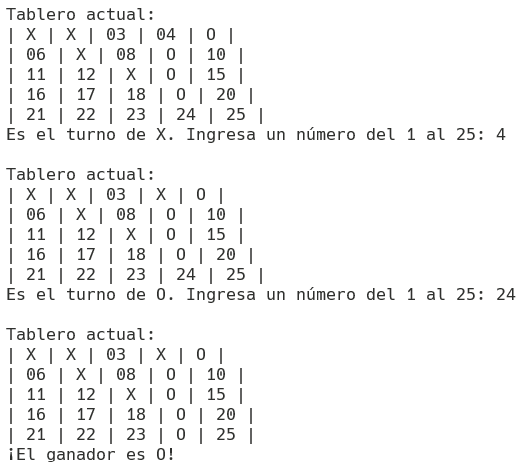
\includegraphics[width=0.8\columnwidth, center]{P1.png}
  \end{figure}

  \subsection*{Problema 2}
  Realice un verificador de contraseña usando encapsulamiento de tipo \textit{private} y \textit{protected}. El programa recibe una cadena candidata para ser contraseña y se valida que:
  \begin{enumerate}[label=\alph*.]
    \item Tenga entre 8 y 16 de caracteres
    \item Que tenga al menos un carácter especial.
    \item Que tenga al menos un número.
    \item Que tenga al menos una letra minúscula.
    \item Que tenga al menos una letra mayúscula.
  \end{enumerate}
  Investigue como se hace para ocultar los caracteres escritos en la consola.

  Al final regrese si la contraseña es débil, mediana o fuerte.

  \textbf{\textit{Implementar encapsulamiento privado y protegido.}}

  \linejump
  \textbf{Explicación} \\
  Este código consta de dos clases: \textit{Password} y \textit{PasswordInput}. La clase \textit{PasswordInput} contiene un método \textit{main()} que solicita al usuario que ingrese una contraseña. Luego, la clase \textit{Password} se encarga de validar y ocultar esta contraseña. La validación se basa en varios criterios, como la longitud mínima, la presencia de caracteres especiales, números y letras mayúsculas/minúsculas.

  En el método \textit{main()} de la clase \textit{Password}, se inicia el proceso recopilando la contraseña del usuario utilizando la clase \textit{PasswordInput}. Luego, se crea una instancia de la clase \textit{Password} con la contraseña obtenida y se utiliza su método \textit{hidePassword()} para ocultar la contraseña original. Finalmente, se llama al método \textit{validate()} para verificar si la contraseña cumple con los criterios de seguridad y se muestra en la consola un mensaje que indica si la contraseña es ``Fuerte'', ``Media'' o ``Débil'' en función de los resultados de la validación.

  \textbf{Clase \textit{PasswordInput}}
  \begin{lstlisting}
import java.io.Console;

class PasswordInput {
  public static String main(String[] args) {
    Console console = System.console();
    if (console == null) {
      System.out.println("No se puede obtener la consola");
      System.exit(0);
    }

    String password = new String(console.readPassword("Ingresa la password: "));

    return password;
  }
}
  \end{lstlisting}

  \textbf{Clase \textit{Password}}
  \begin{lstlisting}
import java.io.IOException;

public class Password {
  private String password;
  private static final String SPECIAL_CHAR = "!@#$%^&*()-_=+[]{};:'\",.<>/?|\n";
  protected static final int MIN_LENGTH = 8;
  protected static final int MAX_LENGTH = 16;

  public Password(String password) {
    this.password = password;
  }

  public String getPassword() {
    return password;
  }

  public void setPassword(String password) {
    this.password = password;
  }

  public static String validate(String password) {
    int length = password.length();
    boolean hasSpecialChar = false;
    boolean hasNumber = false;
    boolean hasUppercase = false;
    boolean hasLowercase = false;

    for (int i = 0; i < length; i++) {
      char c = password.charAt(i);

      if (!hasSpecialChar && SPECIAL_CHAR.indexOf(c) != -1) {
        hasSpecialChar = true;
      }
      if (!hasNumber && Character.isDigit(c)) {
        hasNumber = true;
      }
      if (!hasUppercase && Character.isUpperCase(c)) {
        hasUppercase = true;
      }
      if (!hasLowercase && Character.isLowerCase(c)) {
        hasLowercase = true;
      }
    }

    if (length <= MAX_LENGTH && length > MIN_LENGTH && 
          hasSpecialChar && hasNumber && hasUppercase && hasLowercase) {
      return "Fuerte";
    } else if (length >= 8
          && ((hasUppercase && hasLowercase) || 
          (hasUppercase || hasLowercase) && hasNumber) && hasSpecialChar) {
      return "Media";
    } else {
      return "Debil";
    }
  }

  public static String hidePassword(String password) {
    return "*".repeat(password.length());
  }

  public static void main(String[] args) throws IOException {
    String password = PasswordInput.main(args);

    Password pwd = new Password(password);
    System.out.println("Password oculta: " + hidePassword(pwd.getPassword()));
    System.out.println("La Password es de nivel: " + validate(pwd.getPassword()));
  }
}
  \end{lstlisting}

  \textbf{Ejecución}
  \begin{figure}[ht]
    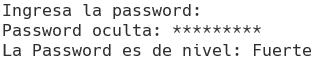
\includegraphics[width=0.6\columnwidth, center]{P2.png}
  \end{figure}

  \subsection*{Problema 3}
  Programa un ahorcado utilizando la composición de objetos:
  \begin{enumerate}[label=\alph*.]
    \item La palabra adivinanza tiene que ser seleccionada de manera aleatoria de un arreglo de mínimo 30 palabras.
    \item El ahorcado deberá mostrarte en consola con una figura simple por ejemplo
    
    Palabra oculta: “MATEMATICAS” \\
    Adivina: $\_$ $\_$ $\_$ $\_$ $\_$ $\_$ $\_$ $\_$ $\_$ $\_$ $\_$

    \begin{figure}[ht]
      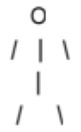
\includegraphics[width=0.15\columnwidth, center]{ahorcado.png}
    \end{figure}
    \item Si el usuario gana mostrar un mensaje de ganador y de la misma manera si se pierde.
    \item Considere las clases:
    \begin{enumerate}[label=\roman*.]
      \item Palabra (palabras ocultas)
      \item Ahorcado (figura)
      \item \textit{Main} (se programa la lógica del juego)
    \end{enumerate}
  \end{enumerate}

  \textbf{\textit{Implementar composición de objetos.}}

  \linejump
  \textbf{Explicación} \\
  Para programar el juego de ahorcado se utilizaron las 3 clases sugeridas. La clase \textit{Palabra} se encarga de elegir aleatoriamente una palabra entre las 30 posibles para crear dos variables, una con la palabra que se tiene que adivinar y otra con guiones bajos ($\_$) que el usuario ira llenando con sus intentos. Esta clase tiene dos métodos \textit{getters} para saber la palabra y la palabra escondida y otro método para comprobar si la letra que ingresó el usuario esta en la palabra original para agregar la letra a la palabra escondida. 
  
  La clase \textit{Ahorcado} se encarga de dibujar la figura simple del ahorcado y también lleva un control de las vidas del jugador por medio de un método \textit{get} y uno para restar una vida en caso de equivocarse. 

  En la clase \textit{Main} se realiza la composición de objetos de las clases \textit{Palabra} y \textit{Ahorcado}. Dentro de un ciclo \textit{while} se muestra la palabra escondida con el progreso que lleva el jugador además de la figura del ahorcado. Se pide una letra y se revisa si está en la palabra original, y en caso de que no esté se resta una vida. El ciclo \textit{while} se interrumpe cuando se acabaron las vidas o si se adivinó la palabra. Por último se imprime un mensaje de victoria o derrota dependiendo el caso. 
    
  \textbf{Clase \textit{Palabra}}
  \begin{lstlisting}
import java.util.Random;

public class Palabra {
  private StringBuilder word = new StringBuilder();
  private StringBuilder hiddenWord = new StringBuilder();
  private Random rand = new Random();

  public Palabra() {
    int r = rand.nextInt(30);
    this.word = new StringBuilder(chooseWord(r).toUpperCase());
    
    for(int i = 0; i < word.length(); i++)
      this.hiddenWord.append('_');
  }

  private String chooseWord(int r) {
    switch(r) {
      case 1: return "personas";
      case 2: return "computadora";
      case 3: return "ciudad";
      case 4: return "sistema";
      case 5: return "historia";
      case 6: return "internet";
      case 7: return "perro";
      case 8: return "gato";
      case 9: return "casa";
      case 10: return "dia";
      case 11: return "noche";
      case 12: return "importante";
      case 13: return "pelicula";
      case 14: return "musica";
      case 15: return "libro";
      case 16: return "desarrollo";
      case 17: return "tiempo";
      case 18: return "programacion";
      case 19: return "cuerpo";
      case 20: return "problema";
      case 21: return "solucion";
      case 22: return "informacion";
      case 23: return "movimiento";
      case 24: return "lenguaje";
      case 25: return "actividad";
      case 26: return "luz";
      case 27: return "fuerza";
      case 28: return "nuevo";
      case 29: return "espacio";
      default: return "naturaleza";
    }
  }

  public StringBuilder getWord() {
    return this.word;
  }

  public StringBuilder getHiddenWord() {
    return this.hiddenWord;
  }

  public boolean guessLetter(char l) {
    boolean inWord = false;
    
    for(int i = 0; i < word.length(); i++) {
      if(word.charAt(i) == l) {
        this.hiddenWord.setCharAt(i, l);
        inWord = true;
      }
    }
    
    return inWord;
  }
}    
  \end{lstlisting}

  \textbf{Clase \textit{Ahorcado}}
  \begin{lstlisting}
public class Ahorcado {
  private int lives = 7;

  public void paintAhorcado() {
    for(int i = 0; i < lives; i++) {
      switch(i) {
        case 0: System.out.print("  O"); break;
        case 1: System.out.print("\n/"); break;
        case 2: System.out.print(" | "); break;
        case 3: System.out.print((char)92); break;
        case 4: System.out.print("\n  |"); break;
        case 5: System.out.print("\n/   "); break;
        case 6: System.out.print((char)92); break;
      }
    }
  }

  public int getLives() {
    return this.lives;
  }

  public void loseLife() {
    this.lives--;
  }
}  
  \end{lstlisting}

  \textbf{Clase \textit{Main}}
  \begin{lstlisting}
import java.util.Scanner;

public class Main {
  public static void main(String[] args) {
    Scanner sc = new Scanner(System.in);
    Ahorcado game = new Ahorcado();
    Palabra p = new Palabra();
    StringBuilder w = new StringBuilder(p.getWord());

    while(game.getLives() > 0 && !p.getHiddenWord().toString().equals(w.toString())) {
      System.out.println("Adivina: " + p.getHiddenWord());
      game.paintAhorcado();

      System.out.print("\nLetra: ");
      char l = sc.next().charAt(0);
      l = Character.toUpperCase(l);
      if(!p.guessLetter(l))
        game.loseLife();
      System.out.println();
    }

    if(game.getLives() == 0)
      System.out.println("Perdiste :( La palabra era: " + w + "");
    else
      System.out.println("Adivinaste la palabra " + w + "!");

    sc.close();
  }
}    
  \end{lstlisting}
  
  \newpage
  \textbf{Ejecución}
  \begin{figure}[ht]
    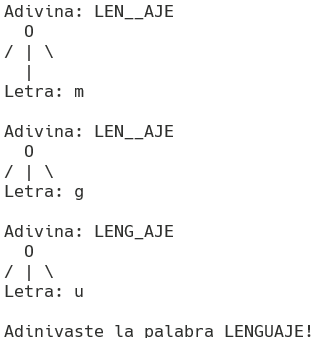
\includegraphics[width=0.6\columnwidth, center]{P3.png}
  \end{figure}

  \subsection*{Problema 4}
  El matemático S. Ulam en 1964 planteo una secuencia de números entera que sigue una serie de reglas planteada en \url{https://edabit.com/challenge/RkicZ4kkcSx8K3d4e}x. Programe la secuencia de Ulam, pero que reciba desde consola los primeros dos elementos de la secuencia y se calcule sobre esos dos elementos.

  Por ejemplo:
  \begin{figure}[ht]
      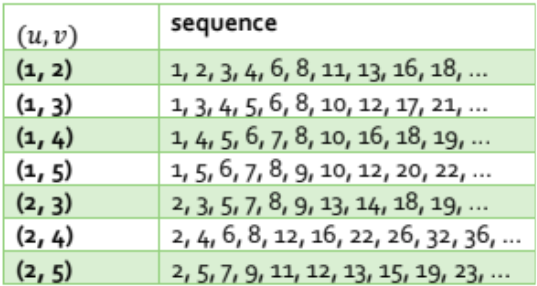
\includegraphics[width=0.8\columnwidth, center]{secuencia.png}
  \end{figure}

  \textbf{\textit{Para manejar la secuencia haga uso de ArrayList exclusivamente.}}

  \linejump
  \textbf{Explicación} \\
  El programa funciona a partir de los dos primeros números de la secuencia ingresados en la consola, los cuales se envían al método \textit{ulam} que se encarga de calcular los siguientes 8 números.

  En el método se utiliza la colección \textit{ArrayList} para crear dos variables, la secuencia (\textit{sequence}) y la suma de los elementos de la secuencia (\textit{sums}). Primero se agregan los dos números ingresados por el usuario, luego, dentro de un ciclo \textit{for}, se vacia la variable \textit{sums} para volver a llenarla con los sumas de los elementos de la secuencia. Después, utilizando el método \textit{sort} y la clase \textit{Comparator} se ordena la lista de sumas para eliminar los elementos de \textit{sums} que ya están en la secuencia.

  Por último, dentro de un ciclo \textit{while} se busca a la suma menor y que no este repetida a través de dos condicionales. La primera solo se aplica cuando la lista de sumas tiene un elemento, pues no tiene más con que comparar. La segunda comprueba si un elemento de \textit{sums} está repetido, y si lo está procede a eliminar todas las repeticiones de este número. Si no se cumplieron las dos condicionales quiere decir que el elemento en 0 de \textit{sums} es la suma mínima y no repetida y se agrega a la secuencia. Al terminar con los 8 elementos de la secuencia, se retorna y se imprime en el método \textit{main}.

  \textbf{Código}
  \begin{lstlisting}
import java.util.Scanner;
import java.util.ArrayList;
import java.util.Comparator;

public class Problema4 {
  static ArrayList<Integer> ulam(int u, int v) {
    ArrayList<Integer> sequence = new ArrayList<Integer>();
    ArrayList<Integer> sums = new ArrayList<Integer>();

    sequence.add(u);
    sequence.add(v);

    for(int i = 0; i < 8; i ++) {
      sums.clear();

      for(int j = 0; j < sequence.size(); j ++) {
        for(int k = j + 1; k < sequence.size(); k ++)
          sums.add(sequence.get(j) + sequence.get(k));
      }

      sums.sort(Comparator.naturalOrder());

      for(int j = 0; j < sums.size(); j ++) {
        if(sequence.contains(sums.get(j))) {
          sums.remove(j);
          j --;
        }
      }

      while(true) {
        if(sums.size() == 1) {
          sequence.add(sums.get(0));
          break;
        } else if(sums.get(0) == sums.get(1)) {
          int temp = sums.get(0);
          while(sums.get(0) == temp)
            sums.remove(0);
        } else {
          sequence.add(sums.get(0));
          break;
        }
      }
    }

    return sequence;
  }

  public static void main(String[] args) {
    Scanner sc = new Scanner(System.in);

    System.out.print("Numero 1: ");
    int u = sc.nextInt();
    System.out.print("Numero 2: ");
    int v = sc.nextInt();


    System.out.println("\nPrimeros 10 numeros de la secuencia: ");
    System.out.println(ulam(u, v));

    sc.close();
  }
}    
  \end{lstlisting}

  \textbf{Ejecución}
  \begin{figure}[ht]
    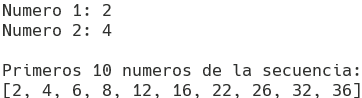
\includegraphics[width=0.6\columnwidth, center]{P4.png}
  \end{figure}

  \section*{Conclusiones}
  La aplicación efectiva de los principios de abstracción y encapsulamiento en el diseño de clases y sistemas de software es esencial para crear soluciones sólidas y mantenibles. La abstracción nos permite centrarnos en lo que hace una clase sin preocuparnos por cómo lo hace, simplificando así la comprensión y el uso de objetos complejos. Por otro lado, el encapsulamiento protege la información interna de una clase y oculta su implementación, lo que garantiza la integridad de los datos y reduce la complejidad del código.

  Estos principios también promueven la modularidad, la reutilización de código y la colaboración efectiva en proyectos de desarrollo de software. Además, mejoran la seguridad al restringir el acceso a datos sensibles y permiten cambios en la implementación sin afectar a otras partes del sistema.


  \section*{Referencias}
  \small
  Solano, J. (2017, 20 enero). \textit{Manual de prácticas de Programación Orientada a Objetos}. Laboratorio de Computación Salas A y B. \url{http://lcp02.fi-b.unam.mx/} \\

  Matt. \textit{Ulam Sequence}. Edabit. \url{https://edabit.com/challenge/RkicZ4kkcSx8K3d4e} \\

  \textit{Java ArrayList sort()}. (n.d.). \url{https://www.programiz.com/java-programming/library/arraylist/sort}x
\end{document}